% questions.tex —— 1977 年·江苏连云港市初试卷 · 题目内容片段（无答案）
% 由 tools/generate_projects.py 依来源总账自 1977/1977_数学真题_江苏连云港市初试_试题.md 生成，勿手改（改源 MD 后重跑）


\gkpart{江苏连云港市初试卷}

\begin{gktip}
\textbf{来源说明}：本题面依据固定源 PDF《1977江苏连云港市初试》全部 3 页逐题转录。源 PDF 为 1977 年高考试题汇编的书页扫描，首页顶部印有汇编章节标题「六、连云港市」（原书排版字间有空格），本库 H1 按此标题逐字转写；第 1 页左下角可见原书页码 240，第 2、3 页未见页码。原卷大题以中文数字「一、」至「八、」编号，本库统一转写为 \texttt{\textbf{N．}}；大题一、二、三内部小题原用阿拉伯数字「1.2.3.」编号，本库转写为全角括号 \texttt{（N）}，其中大题一第（2）小题原卷用「(1)(2)」为两个数列小项编号，为避免与小问括号重复，本库改用「①②」区分（先例见 1977 天津卷第 1 题）；大题五、六内部小题原卷已用全角括号「（1）（2）」，直接沿用。原卷第四大题标题印作「求极根」，据其后所接极限记号 $\lim\limits_{n\to\infty}[\cdots]$ 判断，当为「求极限」之排印讹误，本文按原卷字面保留并见源注。原卷末尾「附加题」无独立编号，本库续接主体题号记为「附加题 9」，不计入正式题量。扫描件为纯题面材料，未附答案；配套答案与解析为本库编者独立推导，\textbf{非官方标准答案}。
\end{gktip}

\par\medskip

\begin{question}
\gkti{1}填充（每空 2 分）：

（1） 把指数式 $3^2=9$ 改写成对数式 $\underline{\hspace{3em}}$。

（2） 写出下列数列的通项公式：

① $2,4,6,8,10,\cdots\cdots$，$a_n=\underline{\hspace{2em}}$；

② $-1,1,-1,1,\cdots\cdots$，$a_n=\underline{\hspace{2em}}$；

（3） 以点 $(0,0)$ 为圆心，以 $4$ 为半径的圆的方程是 $\underline{\hspace{3em}}$。

\end{question}
\begin{question}
\gkti{2}计算：

（1） $1^{0.123}\times\left(\dfrac32\right)^{-3}\div\left(-\dfrac9{10}\right)^0$；

（2） $\log_{27}81-\lg100$；

（3） $\dfrac{\sqrt[3]{x^{\frac72}\sqrt{x^{-1}}}}{\sqrt{\sqrt[3]{x^{-7}}\sqrt[3]{x^{13}}}}$；

（4） $\dfrac{\left(\sin22^\circ30'+\cos22^\circ30'\right)^2}{2\cos0^\circ-2\sin15^\circ\cos15^\circ+\sin270^\circ}$。

\end{question}
\begin{question}
\gkti{3}对于下列函数，写出自变量 $x$ 的取值范围：

（1） $y=\dfrac{6x-1}{2x-1}$；

（2） $y=\sqrt{x}+\sqrt{-x}$；

（3） $y=\sqrt{\lg\dfrac12(x+1)}$。

\end{question}
\begin{question}
\gkti{4}求极根

\nopagebreak[4]
\[
\lim_{n\to\infty}\left[\frac{1+3+5+\cdots\cdots+(2n-1)}{n+2}-n\right].
\]

\begin{gktip}
\textbf{源注}：原卷本大题标题印作「求极根」，据后接极限记号 $\lim\limits_{n\to\infty}[\cdots]$ 判断，当为「求极限」之排印讹误；本文按原卷字面保留，解析按「求极限」处理。
\end{gktip}

\end{question}
\begin{question}
\gkti{5}

（1） $k$ 为何值时，方程 $x^2-2kx+3=0$ 有一个根是 $-2$？

（2） 试判别一元二次方程 $ax^2+(a-b)x-(a+b)=0$ 的根的情况。

\Needspace{0.4\textheight}
\end{question}
\begin{question}
\gkti{6}已知椭圆

\nopagebreak[4]
\[
\frac{x^2}{5^2}+\frac{y^2}{3^2}=1,
\]

（1） 求此椭圆的长轴的长、离心率、焦点坐标和准线方程；

（2） 如图过椭圆的一个焦点 $F$，作 $FA$ 平行于 $Y$ 轴交椭圆的上半部于 $A$ 点，求 $A$ 点的坐标；
\nopagebreak[4]
\begin{center}% 1977 年江苏连云港市初试卷第 6 题：椭圆 x²/5²+y²/3²=1，
% 焦点 F 在正 X 轴上，过 F 作 FA 平行于 Y 轴交椭圆上半部于 A，标出三角形 AOF（按源卷第 2 页布局）
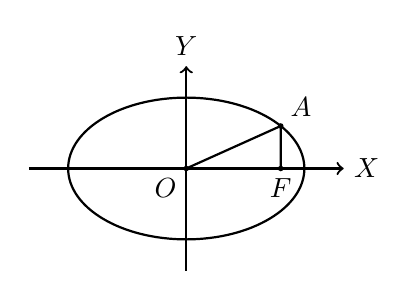
\begin{tikzpicture}[scale=1]
  \draw[thick,->] (-2,0) -- (2,0) node[right] {$X$};
  \draw[thick,->] (0,-1.3) -- (0,1.3) node[above] {$Y$};
  \draw[thick] (0,0) ellipse (1.5 and 0.9);
  \coordinate (O) at (0,0);
  \coordinate (F) at (1.2,0);
  \coordinate (A) at (1.2,0.54);
  \draw[thick] (O) -- (A) -- (F);
  \fill (O) circle (1pt) node[below left] {$O$};
  \fill (F) circle (1pt) node[below] {$F$};
  \fill (A) circle (1pt) node[above right] {$A$};
\end{tikzpicture}
\end{center}
\nopagebreak[4]
（3） 求 $\triangle AOF$ 的面积。

\Needspace{0.4\textheight}
\end{question}
\begin{question}
\gkti{7}如图：把小矩形 $ABCD$ 扩充为大矩形 $AEFG$，并使 $BE+EF+FG+GD=22$，已知小矩形的宽 $AB=2$，小矩形的周长为 $12$，问 $BE$ 为何值时扩充部分的面积最大？最大面积是多少？（扩充部分为图中阴影部分）
\nopagebreak[4]
\begin{center}% 1977 年江苏连云港市初试卷第 7 题：小矩形 ABCD 扩充为大矩形 AEFG，
% 阴影（斜线填充）部分为扩充增加的面积（按源卷第 2—3 页「第七题图」布局）
\begin{tikzpicture}[scale=1]
  \coordinate (A) at (0,2.8);
  \coordinate (D) at (1.6,2.8);
  \coordinate (G) at (2.8,2.8);
  \coordinate (B) at (0,2.0);
  \coordinate (C) at (1.6,2.0);
  \coordinate (E) at (0,0);
  \coordinate (F) at (2.8,0);
  \path[pattern=north east lines, even odd rule] (E) rectangle (G) (B) rectangle (D);
  \draw[thick] (A) -- (G) -- (F) -- (E) -- cycle;
  \draw[thick] (A) -- (D) -- (C) -- (B) -- cycle;
  \fill (A) circle (1.2pt) node[above left] {$A$};
  \fill (D) circle (1.2pt) node[above] {$D$};
  \fill (G) circle (1.2pt) node[above right] {$G$};
  \fill (B) circle (1.2pt) node[left] {$B$};
  \fill (C) circle (1.2pt) node[above right] {$C$};
  \fill (E) circle (1.2pt) node[below left] {$E$};
  \fill (F) circle (1.2pt) node[below right] {$F$};
\end{tikzpicture}
\end{center}
\nopagebreak[4]
\Needspace{0.4\textheight}
\end{question}
\begin{question}
\gkti{8}已知 $AD$ 是 $\odot O$ 的弦，且 $AD=8$，半径 $OH\perp AD$，交 $AD$ 于 $B$ 点，且 $HB=2$，又 $AC$ 是圆的直径，试求 $BC$ 的长。
\nopagebreak[4]
\begin{center}% 1977 年江苏连云港市初试卷第 8 题：⊙O 中弦 AD、直径 AC，
% 半径 OH⊥AD 交 AD 于 B，求 BC 的长（按源卷第 3 页「第八题」布局，AB=BD=4、OB=3、半径=5 等比例缩放）
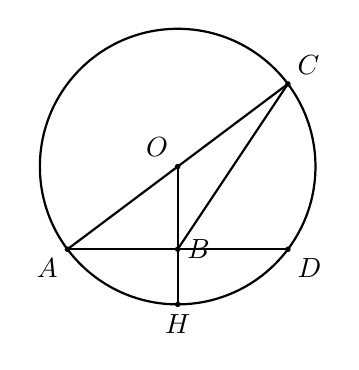
\begin{tikzpicture}[scale=1]
  \coordinate (O) at (0,0);
  \coordinate (A) at (-1.4,-1.05);
  \coordinate (D) at (1.4,-1.05);
  \coordinate (H) at (0,-1.75);
  \coordinate (C) at (1.4,1.05);
  \coordinate (B) at (0,-1.05);
  \draw[thick] (O) circle (1.75);
  \draw[thick] (A) -- (D);
  \draw[thick] (A) -- (C);
  \draw[thick] (O) -- (H);
  \draw[thick] (B) -- (C);
  \fill (O) circle (1pt) node[above left] {$O$};
  \fill (A) circle (1pt) node[below left] {$A$};
  \fill (D) circle (1pt) node[below right] {$D$};
  \fill (H) circle (1pt) node[below] {$H$};
  \fill (C) circle (1pt) node[above right] {$C$};
  \fill (B) circle (1pt) node[right] {$B$};
\end{tikzpicture}
\end{center}
\nopagebreak[4]
\textbf{附加题 9．} 如图 $A$ 是双曲线 $x^2-y^2=1$ 上的一点，$A$ 点处的法线交坐标轴于 $B$、$C$ 两点，若 $|BC|=42$，试求 $|OA|$。

\begin{gktip}
\textbf{提示}：设 $A(x_0,y_0)$，先求出法线斜率，次写出方程，找出 $B$、$C$ 坐标，再用距离公式求出 $A$ 点坐标。
\end{gktip}
\nopagebreak[4]
\begin{center}% 1977 年江苏连云港市初试卷附加题（第 9 题）：双曲线 x²-y²=1 上一点 A，
% A 点处法线交坐标轴于 B（Y 轴）、C（X 轴），B、A、C 三点共线（按源卷第 3 页「附加题」布局，取样例点示意）
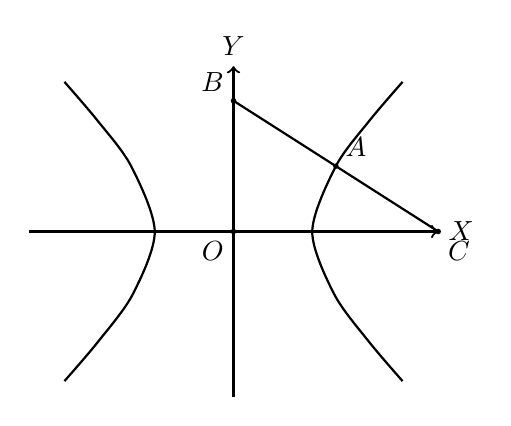
\begin{tikzpicture}[scale=1]
  \draw[thick,->] (-2.6,0) -- (2.6,0) node[right] {$X$};
  \draw[thick,->] (0,-2.1) -- (0,2.1) node[above] {$Y$};
  \draw[thick] plot[smooth] coordinates {(2.147,-1.9) (1.720,-1.4) (1.281,-0.8) (1,0) (1.3,0.83) (1.720,1.4) (2.147,1.9)};
  \draw[thick] plot[smooth] coordinates {(-2.147,-1.9) (-1.720,-1.4) (-1.281,-0.8) (-1,0) (-1.3,0.83) (-1.720,1.4) (-2.147,1.9)};
  \coordinate (O) at (0,0);
  \coordinate (B) at (0,1.66);
  \coordinate (A) at (1.3,0.83);
  \coordinate (C) at (2.6,0);
  \draw[thick] (B) -- (C);
  \fill (O) circle (1pt) node[below left] {$O$};
  \fill (B) circle (1pt) node[above left] {$B$};
  \fill (A) circle (1pt) node[above right] {$A$};
  \fill (C) circle (1pt) node[below right] {$C$};
\end{tikzpicture}
\end{center}
\nopagebreak[4]

\end{question}